\clearpage
\section{角色脚下缺少阴影}

维修站里的工具箱在地上有影子，旁边走动的角色却像是悬着的。把场景缩减为一个角色、一块地面和一盏方向光，可以单独检查这束光。两张图取自同一机位和同一姿势，亮度与材质设置相同。先看脚后方的地面，再看手臂和身体之间的暗处。

\begin{center}
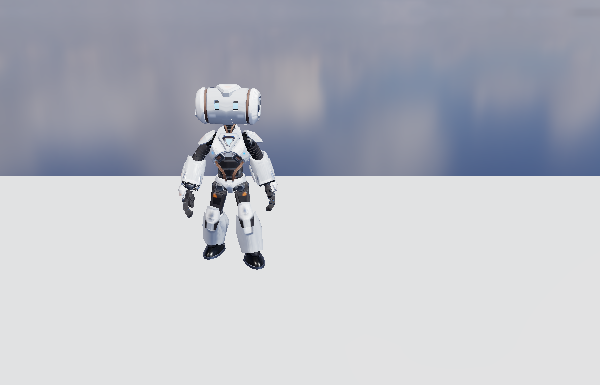
\includegraphics[width=.48\linewidth]{../../../output/validation/animated-shadows/left-off.png}\hfill
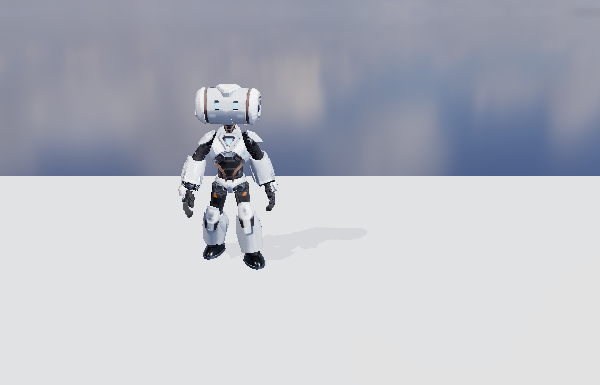
\includegraphics[width=.48\linewidth]{../../../output/validation/animated-shadows/left-on.png}\\
{\small 左图关闭角色阴影，右图使用 $512\times512$ 的光源深度图。均为 Redflag Vulkan 帧，模型源自 Godot 第三人称样例。}
\end{center}

相机能看见角色，只能说明它进入了相机的绘制名单。原来光照还要从地面朝灯发出一条射线，搜索挡在中途的静态三角形。构造这份场景数据时，\texttt{LightingPreview.cpp} 的 \texttt{CollectModels} 碰到有动画的模型便提前返回。把角色的某一帧放进静态数据会在地面留下过时的影子，因此这一步适合烘焙。实时方向光还缺少一份与当前姿势相符的遮挡记录。

现在每盏开启投影的方向光都从自己的位置看向角色。它记录沿照射方向首先碰到的表面深度 $z_c$。画地面时，把地面上的点投影到同一张图上，得到它的深度 $z_r$。如果 $z_c=0.30$、$z_r=0.65$，说明这束光先碰到角色，地面便收不到它。周围建筑和天空反射来的光仍能照亮地面。阴影边缘取附近四格分别比较，按距离合并结果。原理与示意图见 \href{https://learnopengl.com/Advanced-Lighting/Shadows/Shadow-Mapping}{LearnOpenGL《Shadow Mapping》中的 Shadow mapping 与 PCF}。

\begin{Code}
// GI.comp, direct. wi 是从当前表面朝向灯的单位向量。
if (light.p.w == -1.)
    attenuation *= animatedVisibility(id, s.p.xyz, s.n.xyz, wi);
\end{Code}
\loc{Redflag/src/Redflag/Renderer/GI/Shaders/GI.comp}

光源能看见哪些部件由 \texttt{SceneRenderer::DrawGeometry} 决定。它读取角色本帧蒙皮后的网格和各部件的位置。灯移动、角色抬手或换姿势后，\texttt{LightingPreview::DrawAnimatedShadows} 重新绘制；只移动相机时，原先的角色深度仍可使用。编辑器里展开“实时效果”，在“角色阴影”选择图宽。地面与房间的静态遮挡、探针烘焙、环境反射各自沿用已有数据。

把角色沿世界 $X$ 轴移动 1.80 个场景单位，再用 RenderDoc 比较直接光开关前后的线性 RGB。我们统计地面上三个通道的平均亮度至少下降 0.03 的像素，计算这些像素对应的世界坐标均值。两次均值相差 1.81，脚下和手臂周围的阴影都随角色移动。把场景中唯一的灯强度调到零后，直接光输出也降到零。再从左右两侧各打一盏红光和蓝光，地面分别出现只缺红光和只缺蓝光的区域。复现入口为 \path{tests/check_animated_shadows.py}，逐帧记录见 \path{output/validation/animated-shadows/}。
